\documentclass[12pt]{article}

% a template that a friend gave, it's worked well enough for me
% i have added some packages and stuff that have proved useful

\usepackage{fancyhdr}
\usepackage{tipa}
\usepackage{fontspec}
\usepackage{amsfonts}
\usepackage{enumitem}
\usepackage[margin=1in]{geometry}
\usepackage{graphicx}
\usepackage{float}
\usepackage{amsmath}
\usepackage{braket}
\usepackage{amssymb}
\usepackage{booktabs}
\usepackage{hyperref}
\usepackage{mathtools}
\usepackage{xcolor}
\usepackage{float}
\usepackage{algpseudocodex}
\usepackage{titlesec}
\usepackage{bbm}

\pagestyle{fancy}
\fancyhf{} % sets both header and footer to nothing
\lhead{Kevin Sheng}
\setmainfont{Comic Neue}
\renewcommand{\headrulewidth}{1pt}
\setlength{\headheight}{0.75in}
\setlength{\oddsidemargin}{0in}
\setlength{\evensidemargin}{0in}
\setlength{\voffset}{-.5in}
\setlength{\headsep}{10pt}
\setlength{\textwidth}{6.5in}
\setlength{\headwidth}{6.5in}
\setlength{\textheight}{8in}
\renewcommand{\headrulewidth}{0.5pt}
\renewcommand{\footrulewidth}{0.3pt}
\setlength{\textwidth}{6.5in}
\usepackage{setspace}
\usepackage{multicol}
\usepackage{float}
\setlength{\columnsep}{1cm}
\setlength\parindent{24pt}
\usepackage [english]{babel}
\usepackage [autostyle, english = american]{csquotes}
\MakeOuterQuote{"}

\setlength{\parskip}{6pt}
\setlength{\parindent}{0pt}

\titlespacing\section{0pt}{12pt plus 4pt minus 2pt}{0pt plus 2pt minus 2pt}
\titlespacing\subsection{0pt}{12pt plus 4pt minus 2pt}{0pt plus 2pt minus 2pt}
\titlespacing\subsubsection{0pt}{12pt plus 4pt minus 2pt}{0pt plus 2pt minus 2pt}

\hypersetup{colorlinks=true, urlcolor=blue}

\newcommand{\correction}[1]{\textcolor{red}{#1}}


\rhead{Math 180}

\makeatletter
\def\@seccntformat#1{%
  \expandafter\ifx\csname c@#1\endcsname\c@section\else
  \csname the#1\endcsname\quad
  \fi}
\makeatother

\newcommand{\Mod}[1]{\ (\mathrm{mod}\ #1)}

\begin{document}

\section{Chapter 4.4}

\begin{enumerate}
      \item[1] \begin{enumerate}
                  \item If we treat each segment of land as a node and each bridge as an edge,
                        then we have the following degree sequence:
                        \[3, 3, 3, 5\]
                        We can't have any odd-degree vertices if we want an Eulerian tour,
                        so no such tour can exist in this graph.

                        Even if we aren't required to return to the starting point,
                        it's still not possible.
                        For such a path to exist, we can have at most $2$ odd-degree vertices.
                        This can then be converted to a closed tour by simply adding
                        one (1) additional edge between the start and end.
                  \item For a closed tour to exist, we need to add at least $2$ bridges
                        so that all the nodes' degrees are turned even.
            \end{enumerate}
      \item[7] \begin{enumerate}
                  \item All the graphs have Hamiltonian cycles.
                        I've enumerated the nodes in each of them below.
                        \begin{center}
                              \hfill
                              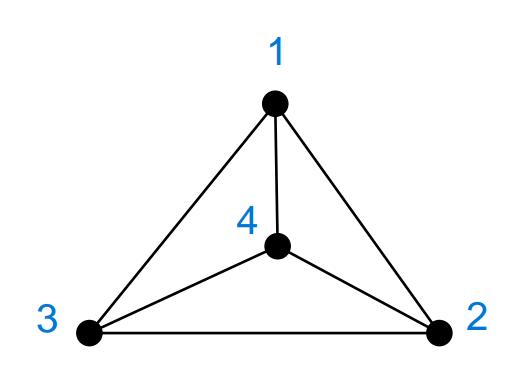
\includegraphics[height=3cm]{img/hw2/hamil1}
                              \hfill
                              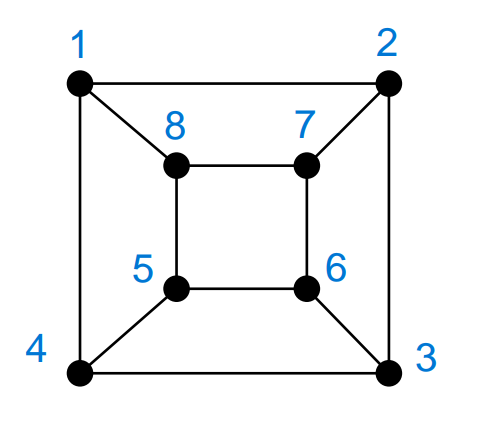
\includegraphics[height=3cm]{img/hw2/hamil2}
                              \hfill
                              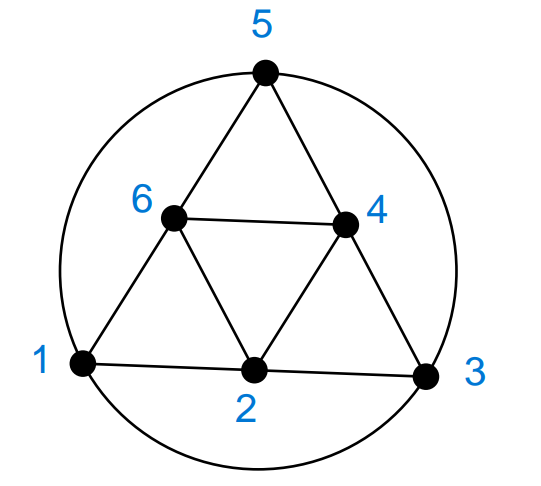
\includegraphics[height=3cm]{img/hw2/hamil3}
                              \hfill \mbox{} \\
                              \hfill
                              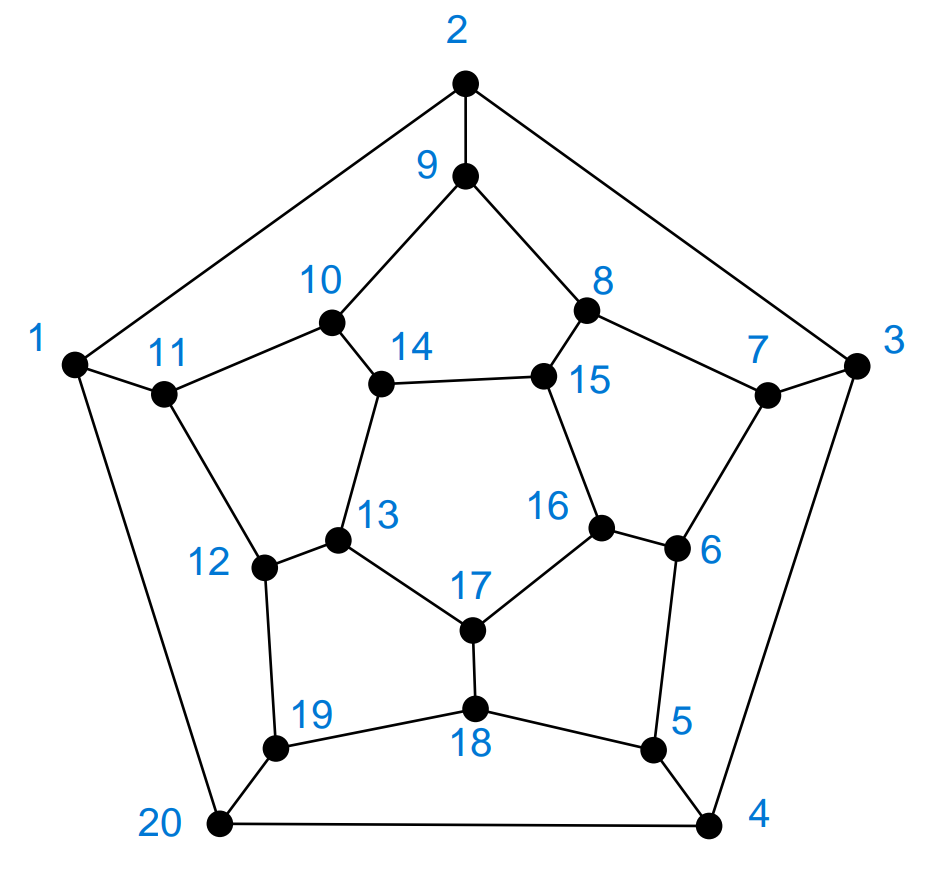
\includegraphics[height=6cm]{img/hw2/hamil4}
                              \hfill
                              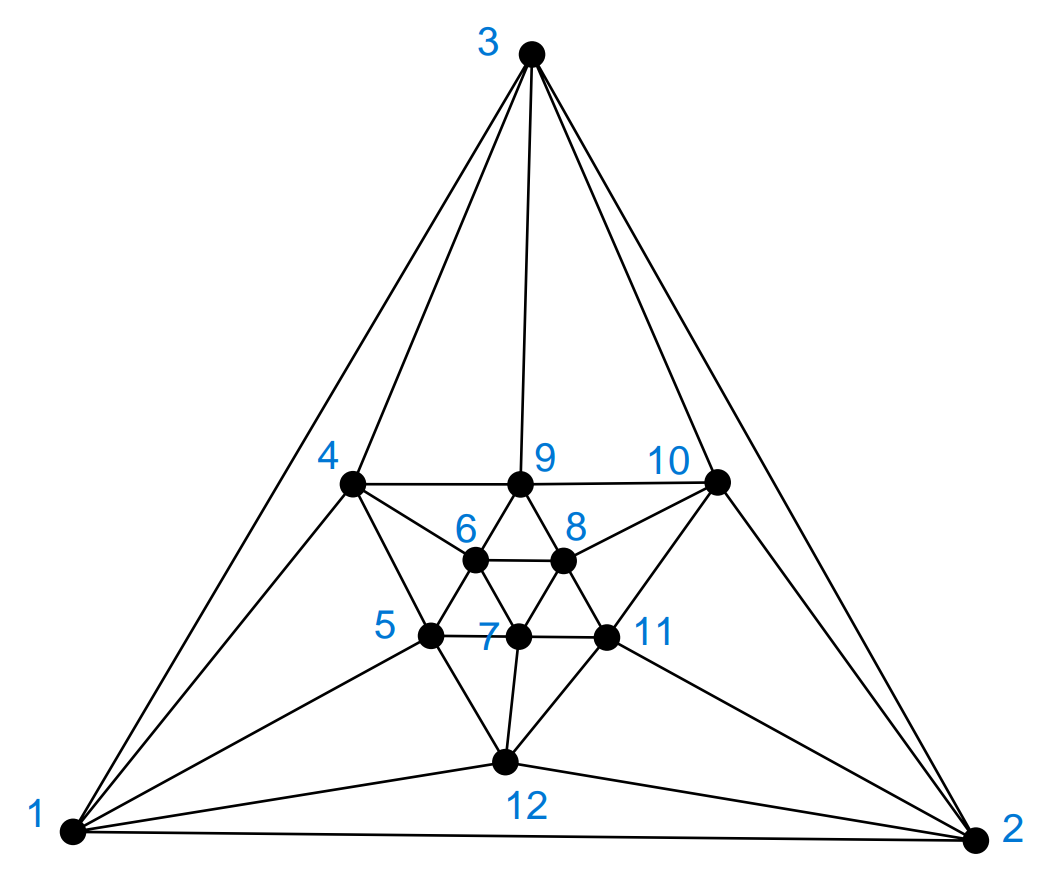
\includegraphics[height=6cm]{img/hw2/hamil5}
                              \hfill \mbox{}
                        \end{center}

                        \pagebreak

                  \item Have the following two graphs:
                        \begin{center}
                              \hfill
                              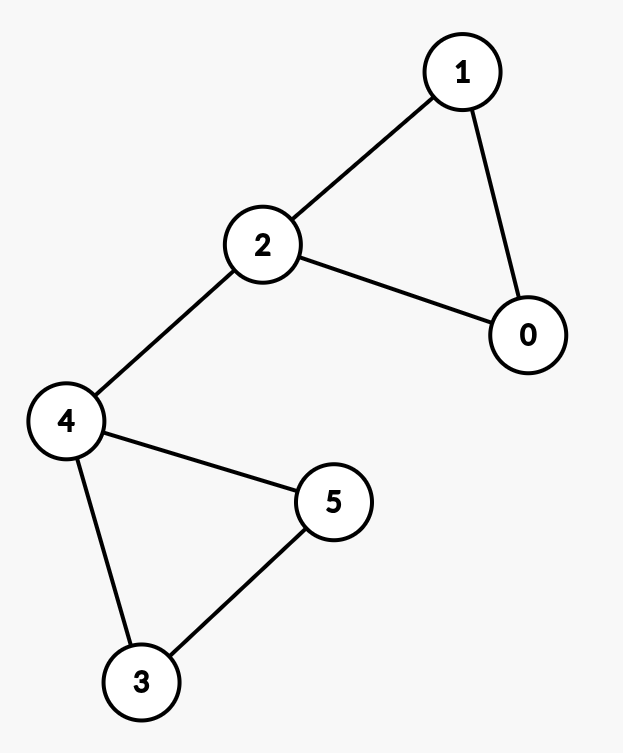
\includegraphics[height=6cm]{img/hw2/has_cycle}
                              \hfill
                              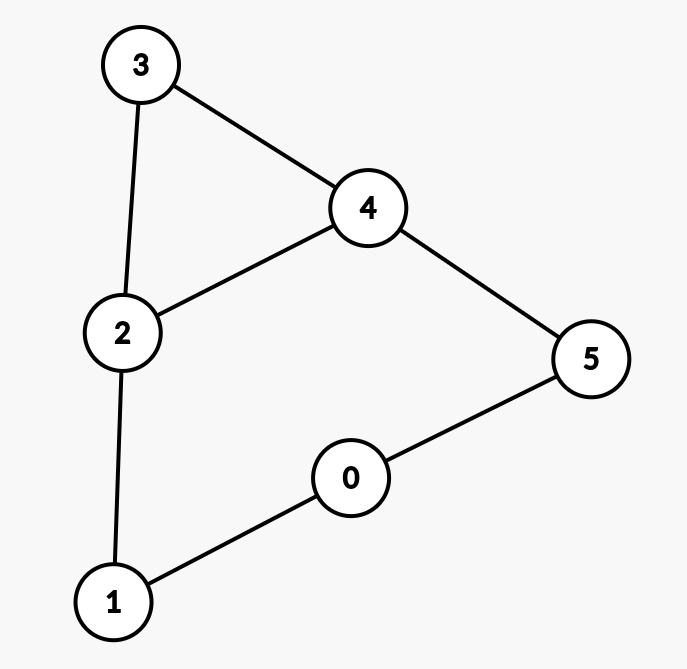
\includegraphics[height=6cm]{img/hw2/has_no_cycle}
                              \hfill \mbox{}
                        \end{center}
                        Both have the degree sequence
                        \[2, 2, 2, 2, 3, 3\]
                        but only the right graph has a Hamiltonian cycle.
            \end{enumerate}
\end{enumerate}

\pagebreak

\section{Chapter 4.5}

\begin{enumerate}
      \item[1] \textbf{Necessity} \\
      If the graph isn't even weakly connected, then there's no chance
      we can jump from one component to another.
      Also, we need the indegree of each node to be equivalent to the outdegree
      because in an Eulerian tour, we're always entering and leaving each
      node the same amount of times, including the start.

      \textbf{Sufficience} \\
      Like with the original proof of the condition for an Euler Tour,
      let's start with a tour of the largest possible length and show that
      we can always extend it until it becomes an Euler Tour.
      \begin{itemize}
            \item If it isn't closed, the starting node must have an ingoing
            edge that isn't used yet since we left it one more time
            than we entered it.
            Thus, we can always push the start back until we make it a closed loop.
            \item Say our tour consists of all nodes in the set $V(T)$.
            If $\exists v \in V: v \notin V(T)$, by weak connectivity
            $\exists v' \in V(T): (v, v') \in E \lor (v', v) \in E$. \\
            In both cases, we can add on $v$ to the tour by putting it at the
            front or back, depending on whether the edge goes into or out of $v$.
            \item Now, suppose the edges our tour has visited is $E(T)$.
            If $E(T) \ne E$, by the same reasoning as the proof of the original
            degree condition for an Euler Tour we can always add on this new edge.
      \end{itemize}
      From this, we can see that any tour in a directed graph satisfying the
      given conditions can be turned into an Euler Tour. $\square$

      \item[6] \textbf{(i) implies (ii)} \\
      First, assign alternating colors to every node of the even cycle.
      We'll have the two colors be red and blue, because why not?

      Then, for all other nodes in the graph, consider the parity
      of their closest distance to any red node in the cycle.
      We can reach the cycle in the first place since the graph is strongly connected.
      Assign blue to nodes with odd distance, and red to those with even distance.

      To prove that this is a valid coloring, suppose for sake of contradiction
      that this method resulted in a node $v$ with the same color as all the nodes it's connected to.
      This means
      \[\text{dist}(v) \equiv \text{dist}(u) \Mod 2\ \forall u \in V: (v, u) \in E\]
      but this can't be true, since $\exists (v, u) \in E: \text{dist}(v)=\text{dist}(u)+1$
      by how we defined distance.
      Thus, our coloring must be valid.

      \textbf{(ii) implies (i)} \\
      Suppose there exists a valid coloring.
      Start at an arbitrary node $v$ and go to any other node $v'$
      that has a different color from $v$.
      Repeat this process until we hit a node that we've already discovered.
      Since the graph is strongly connected, this is guaranteed to happen.

      This gives us a node sequence that looks like:
      \[v_1, v_2, \cdots, v_i, \cdots, v_j, v_i\]
      where any two nodes that are adjacent in the sequence have different colors.
      
      Since the colors in the cycle we constructed from $v_i$ to $v_i$
      must be alternating, it has to be of even length as well. $\square$

      \item[8] Consider a path $v_1, \cdots, v_n$ of length $n$.
      We WTS that $n \ne |V|$ then it isn't the longest path.
      This then implies the existence of a path of length $|V|$
      that includes all the vertices, since a longest path has to
      exist in every graph.

      BWOC say that it actually was.
      Then $\exists v \in V$ that isn't in our path.
      Since this is a tournament graph,
      $\forall i=1, \cdots, n\ (v, v_i) \in E \lor (v_i, v) \in E$.
      For each $i$, let's call it \textit{ingoing} if the edge goes from $v$ to it
      and \textit{outgoing} otherwise.

      If $v_1$ is ingoing, we can add $v$ to the start of the path.
      OTOH, if $v_n$ is outgoing, we can append $v$ to our path.
      This leaves the case where $v_1$ is outgoing and $v_n$ is ingoing.

      Notice that $\exists 1 \le i \le n$ where $v_i$ is outgoing and $v_{i+1}$ is ingoing.
      Such a point is guaranteed because we start at $v_1$ which is outgoing
      and end at $v_n$ which is ingoing.
      Given this, we can add $v$ to the path like so:
      \[v_1, \cdots, v_i, v, v_{i+1}, \cdots, v_n\]
      
      In all three cases, we can always add $v$ to our path,
      and so any path that doesn't include all nodes isn't a longest path. $\square$
\end{enumerate}

\end{document}
